\documentclass[11pt]{report}
\usepackage[utf8]{inputenc}
\usepackage[margin=1in]{geometry}
\usepackage{amsfonts,amsmath,amssymb}
\usepackage[none]{hyphenat}
\usepackage[utf8]{inputenc}
\usepackage{fancyhdr}
\usepackage{graphicx}
\graphicspath{{images/}}
\usepackage[nottoc, notlot, notlof]{tocbibind}
\usepackage[spanish]{babel}
\usepackage{enumitem}
\usepackage{hyperref}
\usepackage{eurosym}
\usepackage[T1]{fontenc}
\usepackage{listings}
\usepackage{xcolor}
\usepackage{textcomp}
\usepackage{eurosym}


\renewcommand{\UrlFont}{\ttfamily\small}

\pagestyle {fancy}
\fancyhead{}
\fancyfoot{}
\fancyhead[L]{\slshape\MakeUppercase{Trabajo de fin de grado}}
\fancyhead[R]{\slshape Ionut Morariu}
\fancyfoot[C]{\thepage}


\parindent 0ex
%\setlength{\parindent}{4em} %Change indent width
%\setlength{\parskip}{1em} %space between paragraphs

\lstdefinelanguage{JavaScript}{
  morekeywords=[1]{break, continue, delete, else, for, function, if, in,
    new, return, this, typeof, var, void, while, with},
  % Literals, primitive types, and reference types.
  morekeywords=[2]{false, null, true, boolean, number, undefined,
    Array, Boolean, Date, Math, Number, String, Object},
  % Built-ins.
  morekeywords=[3]{eval, parseInt, parseFloat, escape, unescape,console},
  sensitive,
  morecomment=[s]{/*}{*/},
  morecomment=[l]//,
  morecomment=[s]{/**}{*/}, % JavaDoc style comments
  morestring=[b]',
  morestring=[b]"
}[keywords, comments, strings]

\lstalias[]{ES6}[ECMAScript2015]{JavaScript}

\lstdefinelanguage[ECMAScript2015]{JavaScript}[]{JavaScript}{
  morekeywords=[1]{await, async, case, catch, class, const, default, do,
    enum, export, extends, finally, from, implements, import, instanceof,
    let, static, super, switch, throw, try},
  morestring=[b]` % Interpolation strings.
}

% Requires package: color.
\definecolor{mediumgray}{rgb}{0.3, 0.4, 0.4}
\definecolor{mediumblue}{rgb}{0.16, 0.5, 0.73}
\definecolor{forestgreen}{rgb}{0.13, 0.55, 0.13}
\definecolor{darkviolet}{rgb}{0.58, 0.0, 0.83}
\definecolor{royalblue}{rgb}{0.25, 0.41, 0.88}
\definecolor{crimson}{rgb}{0.86, 0.8, 0.24}
\definecolor{lightgrey}{rgb}{0.97, 0.97, 0.97}
\definecolor{black}{rgb}{0.05, 0.05, 0.1}
\definecolor{green}{rgb}{0.1529, 0.6823, 0.3764}
\definecolor{red6}{rgb}{0.753, 0.224, 0.169}

\lstdefinestyle{JSES6Base}{
  backgroundcolor=\color{lightgrey},
  basicstyle=\fontsize{7}{9}\selectfont\ttfamily,
  breakatwhitespace=false,
  breaklines=false,
  captionpos=b,
  columns=fullflexible,
  commentstyle=\color{mediumgray}\upshape,
  emph={},
  emphstyle=\color{crimson},
  extendedchars=true,  % requires inputenc
  fontadjust=true,
  frame=single,
  identifierstyle=\color{black},
  keepspaces=true,
  keywordstyle=\color{mediumblue},
  keywordstyle={[2]\color{darkviolet}},
  keywordstyle={[3]\color{red}},
  numbers=left,
  numbersep=10pt,
  numberstyle=\tiny\color{black},
  rulecolor=\color{black},
  showlines=true,
  showspaces=false,
  showstringspaces=false,
  showtabs=false,
  stringstyle=\color{green},
  tabsize=2,
  title=\lstname,
  upquote=true  % requires textcomp
}

\lstdefinestyle{JavaScript}{
  language=JavaScript,
  style=JSES6Base
}
\lstdefinestyle{ES6}{
  language=ES6,
  style=JSES6Base
}

\begin{document}
\begin{titlepage}



\begin{center}
	
\includegraphics[scale=1]{cabecera}\\
	\vspace*{1cm}
	\Large{\textbf{\MakeUppercase{Universidad Pólitécnica de Madrid}}}\\[3mm]
	\Large{{\MakeUppercase{Escuela técnica de ingeniería y diseño industrial}}}\\[3mm]
	\Large {Grado en Ingeneriería Eléctrica}\\
	\vfill
	\line(1,0){400}\\
	\Large{{\MakeUppercase{Trabajo de fin de grado}}}\\
	\Huge{\textbf{Aplicación web para la estimación del coste de una instalación solar conectada a red}}\\[5mm]
	\Large{Autor: Ionut Cristian Morariu}\\
	\line(1,0){400}\\
	\vfill
\end{center}
\begin{flushright}
\Large {Tutor: Óscar Perpiñán Lamigueiro}\\[3mm]
\Large{Departamento de Ingeniería Eléctrica,\\ Electrónica, Automática y Física aplicada}\\[10mm]
Madrid, \today
\end{flushright}

\end{titlepage}

\renewcommand{\baselinestretch}{1.5} %line spacing
\renewcommand{\labelitemi}{\textbullet}

\tableofcontents
\thispagestyle{empty}
\clearpage

\setcounter{page}{1}


\chapter{Introducción}
\section{Objetivos}
El objetivo de este proyecto es el desarrollo de una aplicación o página web de fácil acceso para todos los usuarios, con la finalidad de ofrecer una estimación inicial del coste y la posible generación de una instalación fotovoltaica doméstica de conexión a red.\\

Para poder llevar a cabo esta estimación, el usuario introducirá unos serie de datos acerca de su emplazamiento y edificación en la que desea situar la instalación, y la aplicación hará todos los cálculos necesarios para ofrecer una aproximación lo más cercana al resultado final teniendo en cuenta todas la variables que puedan intervenir.\\

La aplicación también ofrecerá otros datos de posible interés para el usuario como: el número de paneles que se pueden instalar, la potencia de dichos paneles y la potencia del inversor.\\

La idea de esta aplicación surge de una conversación que tuve con un conocido cuando estaba planificando la construcción de su nueva vivienda, en la cual quería realizar una instalación fotovoltaica para reducir el gasto en la factura de electricidad.\\

En su búsqueda no encontró ningún servicio que fuera lo suficientemente sencillo de entender para una persona sin ningún tipo de conocimiento previo acerca de la generación fotovoltaica, que le aportase la posibilidad de poder personalizar los cálculos a su emplazamiento y planos de construcción.\\

Otro de los puntos clave de la aplicación es que sea de código abierto y gratuita para los usuarios, usando fuentes de información disponibles para cualquier interesado. Todos los pasos y operaciones se podrán obtener, analizar y reutilizar de manera gratuita desde un repositorio de Github \footnote{\textit{Github.com:} Plataforma online de almacenamiento de código y documentación de fuentes abiertas.}.\\


Los objetivos detallados de esta aplicación son los siguientes:
\begin{itemize}
\item Diseñar una interfaz de usuario amigable y sencilla de usar para que la pueda utilizar un gran número de personas sin necesidad de conocimientos sobre energía fotovoltaica.

\item Obtención de los datos de irradiación en el emplazamiento indicado por el usuario mediante el uso de API\footnote{\textit{Application Programming Interface}: conjunto de funciones y procedimientos que ofrece la posibilidad de un software a interaccionar con otro.} externas.
\item Realizar todos los cálculos necesarios para ofrecer una estimación competente de los siguientes datos:

\begin{itemize}

\item Número de paneles que se pueden instalar.
\item Potencia máxima a instalar.
\item Potencia del inversor.
\item Energía eléctrica producida en un año.

\end{itemize}
\end{itemize}
\newpage

\section{Análisis previo de soluciones}

Antes de comenzar el desarrollo del proyecto, dediqué un tiempo a estudiar las soluciones existentes de estimaciones de instalaciones fotovoltaicas existentes en el mercado para decidir si tenía cabida una aplicación como la que se iba a desarrollar.\\

Algunas de las soluciones encontradas fueron:

\begin{enumerate}
\item \textbf{PVSyst - Photovoltaic Software}

El software PVSyst, desarrollado por la empresa suiza con el mismo nombre es quizá el más conocido dentro del ámbito del estudio y la estimación de instalaciones fotovoltaicas. Ofrece una amplia capacidad de personalización de todos los componentes de la instalación.

\item \textbf{CalculationSolar.com}

Es el primer resultado de Google al buscar el término \textit{``calculadora de instalaciones fotovoltaicas''}, por tanto será una de las primeras aplicaciones que una persona que desea realizar una instalación en su vivienda visite.

\item \textbf{SISINFO}

Es una herramienta web diseñada y desarrollada por el Instituto de Energía Solar de la Universidad Politécnica de Madrid. Ha sido y es la herramienta interna utilizada por los ingenieros de dicho instituto.

\end{enumerate}

En el apartado \ref{existing_solutions}  se lleva a cabo un desarrollo mas detallado de las características de las soluciones mencionadas así como sus diferencias con la propuesta de este proyecto.

\section{Aspectos técnicos}

\subsection{Backend}

Para el Backend \footnote{\textit{Backend:} Término utilizado para referirse a la parte de una pagina web encargada de tratar las peticiones del usuario en la página.} se ha empleado una tecnología basada en Javascript llamada NodeJS \footnote{\textit{NodeJS:} Entorno de ejecución basado en el motor de Chrome llamado V8. \url{https://nodejs.org/en/} }, con la ayuda de las librerias ExpressJS\footnote{\textit{ExpressJS:} Framework web para el entorno de NodeJS. \url{https://expressjs.com/es/}} y Mongoose \footnote{\textit{Mongoose:} ORM para las BBDD MongoDB \url{https://mongoosejs.com/}}.   \\
La base de datos que se ha utilizado para almacenar los datos necesarios ha sido MongoDB.

En el servidor se realizan varias tareas relacionadas con los cálculos necesarios. Algunas de estas tareas son:
\begin{itemize}
\item Obtención de los datos de irradiación global media en el plano horizontal para el emplazamiento indicado
\item Proceso completo de cálculo para pasar de la irradiación en el plano horizontal al plano inclinado y orientado según los datos introducidos por el usuario
\item Proceso de obtención de los datos relacionados con el perfil horario de temperatura en el emplazamiento indicado
\item Gestión de las diferentes rutas que constituyen la API.
\end{itemize}

\subsection{Frontend}
 Para el Frontend \footnote{\textit{Frontend:} Término utilizado para referirse a la parte de visual de una web, con la que interactúa el usuario.} de la página se han utilizado las tres tecnologías necesarias para poder desarrollar una pagina web: HTML5, CSS3, Javascript.\\
 
La unica libreria utilizada ha sido Bulma \footnote{\textit{Bulma:} Libreria de componentes CSS. \url{https://bulma.io}} para ahorrar tiempo a la hora de darle un aspecto visual agradable a la página.\\

Esta parte de la página es la encargada de recoger los datos del usuario  y enviarlos al servidor para que se realicen los cálculos. Una vez realizados dichos cálculos, la página mostrará la información relevante al usuario, junto con algunos unos gráficos adicionales.\\

Tanto el backend como el frontend están almacenados en un servidor de Linux ofrecido por la empresa DigitalOcean.\\

Todas las tareas mencionadas tanto en la parte de Backend como en la parte de Frontend se describirán en detalle en la sección \ref{sec:theory}, junto con todos los cálculos en los que se ha basado. 

\newpage

\chapter{Estado del arte}

\section{Situación actual del mercado}

\section{Soluciones existentes y sus carencias} \label{existing_solutions}
\begin{enumerate}
\item \textbf{PVSyst - Photovoltaic Software}

El software PVSyst, desarrollado por la empresa suiza con el mismo nombre es quizá el más conocido dentro del ámbito del estudio y la estimación de instalaciones fotovoltaicas. Ofrece una amplia capacidad de personalización de todos los componentes de la instalación.

PVSyst es capaz de calcular con amplio detalle el diseño y dimensionado del sistema, zonas de sombra, envejecimiento del material, almacenamiento de energía, entre otras opciones.\\

PVSyst se diferencia de la aplicación que se desarrolla en este proyecto en algunos puntos importantes como:
	\begin{itemize}
		\item PVSyst es de pago, con una licencia anual de aproximadamente \euro{952} mientras que mi solución es gratuita.
		\item PVSyst es un programa que se debe instalar en un ordenador de Windows (No funciona en Linux u OSX).
		\item PVsyst es poco intuitivo para un usuario con bajos conocimientos de instalaciones fotovoltaicas.
	\end{itemize}
En resumen, PVSyst es un software mucho mas completo y complejo que la solución que yo propongo, y que va enfocada a un público con una base sólida sobre energía fotovoltaica.
\item Second item
\item Third item
\end{enumerate}


\chapter{Parte teórica y desarrollo del código}
\label{sec:theory}

El proceso de cálculo que se va a seguir para la estimación completa de la instalación fotovoltaica conectada a red es el que se detalla en el libro de Óscar Perpiñán, tutor de este trabajo, denominado Energía Solar Fotovoltaica \cite{esf_book}. También se harán menciones a las presentaciones que se encuentran en el mismo enlace que el libro.\\

A lo largo de este capítulo, se utilizará el término \textbf{aplicación} para referirse a todo el conjunto de código relacionado tanto con proceso de obtención de todos los datos necesario como el de mostrar la información relevante al usuario.

\section{Obtención de datos del usuario}
Como he mencionado anteriormente, el objetivo principal de la aplicación es de realizar todos los cálculos que se necesitan para estimar una instalación fotovoltaica conectada a red, de la manera mas exacta posible,  en un emplazamiento concreto elegido por el usuario. Por tanto, el primer paso que tuve que dar con la aplicación fue la de obtener todos los datos necesarios para realizar dichos calculos.
Estos datos son:
\begin{itemize}
\item Emplazamiento del usuario
\item Área, inclinación, orientación y nivel de suciedad de la superficie de instalación
\end{itemize}
\subsection{Emplazamiento del usuario}
Mas adelante, para poder obtener los datos de irradiación global en el plano horizontal, se necesitan los datos de latitud y longitud del sitio del que se quieren obtener dichos datos. Sin embargo, es poco intuitivo pedirle a un usuario que introduzca sus coordenadas, dado que la mayoría desconocen dichos datos.\\
Por lo tanto, la ruta que he tomado es la de pedirle al usuario su dirección, o una dirección cercana a su localización, y utilizar la API de Google Maps \footnote{\textit{API Google Maps}: Enlace interactivo al que se le pueden enviar los datos de una dirección y devuelve las coordenadas de latitud y longitud de un emplazamiento. \url{https://developers.google.com/maps/documentation/javascript/tutorial} } para convertir dicha dirección en las coordenadas de latitud y longitud que necesito para poder extraer la irradiación que he mencionado antes.\\

Este proceso comienza por recoger los datos de la dirección, municipio y código postal a través del formulario que aparece en la página web.

Estos datos son recogidos en el código a través de un nombre único que han recibido:\\
\begin{lstlisting}[style=ES6, caption={Variables correspondientes a los tres campos}]
const addressInput = document.querySelector('#address');
const cityInput = document.querySelector('#city');
const postalInput = document.querySelector('#postal');
\end{lstlisting}

Una vez que tenemos estos datos recogidos en las variables, podemos pedir a la API de Google Maps las coordenadas de latitud y longitud de dicho emplazamiento encadenando las tres variables y una clave única de identificación,  para obtener un enlace único que se corresponde a dicha localización.\\

\begin{lstlisting}[style=ES6, label={lst:getCoordinates}, caption={Función encargada de solicitar los datos a la API}]
const getCoordinates = async () => {
	const address = addressInput.value.split(' ').join('+');
	const city = cityInput.value;
	const postal = postalInput.value;
	const requestURL = `${googleEndpoint}address=${address},${city},${postal}
										,spain&key=${googleApiKey}`;
	const response = await fetch(requestURL);
	const data = await response.json();
	const info = {
		formattedAdress: data.results[0].formatted_address,
		lat: data.results[0].geometry.location.lat,
		long: data.results[0].geometry.location.lng
	};

	return info;
};
\end{lstlisting}

La función de \textbf{getCoordinates} (\ref{lst:getCoordinates}) recoge el valor de la dirección y reemplaza los espacios con el signo + (formato requerido por la API) y lo concatena con el valor del campo de la ciudad y el código postal. Al final le añade una clave única que identifica la aplicación a la hora de establecer limites de uso y evitar abuso de la API.\\

Una vez creado este enlace único, el código lanza la petición al servicio y retorna con la información que es recogida y se guarda en dos variables \textbf{lat} y \textbf{long} para ser utilizadas posteriormente, a la hora de obtener los datos de irradiación global.

\subsection{Área, inclinación, orientación y nivel de suciedad de la superficie de instalación}

Además de las información de latitud y longitud del emplazamiento, el cálculo de la instalación también requiere de información relacionada con el área, la inclinación, la orientación y el nivel de suciedad de la superficie donde se va a realizar la instalación, para poder realizar una estimación lo mas exacta posible.

Estos valores son recogidos directamente de los campos de la pagina web, al igual que los campos anteriores, sin necesitar ningún trato especial:\\
\begin{lstlisting}[style=ES6, caption={Variables correspondientes a los campos indicados}]
const slope = document.querySelector('#slope');
const area = document.querySelector('#area');
const orientation = document.querySelector('#orientation');
const dirtLevel = document.querySelector('#dirt-level');
\end{lstlisting}

\section{Obtención de la irradiación global media en el plano horizontal}

El primer paso del cálculo de una instalación fotovoltaica es el de conocer la irradiación global media en el plano horizontal para el emplazamiento donde se va a realizar el cálculo. En la sección anterior se obtuvieron las coordenadas de latitud y longitud del emplazamiento introducido por el usuario.\\

En esta sección, se va a obtener la irradiación para las dichas coordenadas utilizando un servicio de ADRASE \footnote{\textit{ADRASE}: Acceso a Datos de irradiación Solar en España \url{http://www.adrase.com/}}, un proyecto realizado por el CIEMAT. Este servicio ofrece de manera gratuita y de uso libre, datos correspondientes a valores medios mensuales de irradiación global en el plano horizontal para toda la geografía española.\\

Los datos están disponibles a través de un mapa interactivo y de unos enlaces personalizados que incluyen la valores de latitud y longitud para los que se desea obtener dicha información. En esos enlaces se ofrecen los datos de irradiación global mínima, media y máxima en el plano horizontal.\\

Con el objetivo de no saturar la pagina de ADRASE y evitar error de funcionamiento de la aplicación debidos a la posibilidad de que la página desaparezca en un futuro, se ha realizado una descarga de los datos de la página, con un intervalo de 0.1 tanto en longitud como en latitud y se han guardado en una base de datos.De esta forma también se reducen los tiempos de cálculo en gran medida al tener un acceso casi instantáneo a los valores medios de irradiación. 
Una explicación detallada de como se ha realizado dicha descarga se incluye en el Anexo. (TODO Anexo con explicación).
\newpage

\section{Cálculo de las componentes de la irradiación solar}

Partiendo de los datos obtenidos en la sección anterior debemos calcular las componentes de irradiación directa y difusa en el plano horizontal y después realizar el paso al plano inclinado.

Un esquema resumido del proceso se indica a continuación:

\begin{figure}[ht]
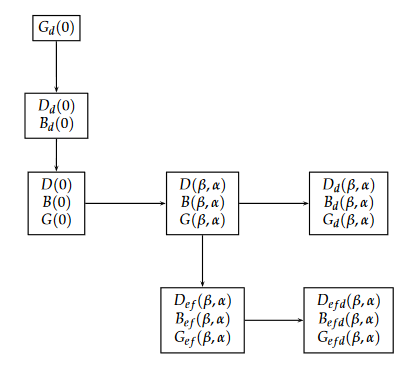
\includegraphics[scale=0.7]{32_ESFBOOK_1}
\centering
\caption{Procedimiendo de cálculo (Figura 3.3 pág 31 \cite{esf_book})}
\label{fig:fig_1}
\end{figure}

En la figura \ref{fig:fig_1} se muestra el proceso de cálculo que se va a seguir para llegar a los valores necesarios para poder estimar la potencia y energía de la instalación.

Los pasos descritos son:
\begin{enumerate}
	\item Separar la irradiación global diaria en el plano horizontal en sus componentes de irradiación difusa y directa.
	\item Convertir la irradiación diaria a un perfil horario de irradiación global, directa y difusa en en plano horizontal.
	\item Pasar del perfil horario en el plano horizontal a un perfil con la inclinación y orientación indicada por el usuario.
	\item Aplicar las pérdidas relacionadas con el ángulo de incidencia y el nivel de suciedad.
	\item Volver a convertir el perfil horario a unos valores diarios de irradiación global, difusa y directa.
\end{enumerate}

\subsection{Separación de la irradiación global diaria en sus componentes}

Como se ha indicado anteriormente, el primer paso del proceso de cálculo es el de separar la irradiación global diaria en en plano horizontal en sus dos componentes, la directa y la difusa.

Al tener solamente un valor de irradiación por cada uno de los meses, utilizaremos el día promedio de cada mes, ya que es posible demostrar que el promedio mensual coincide con el valor diario correspondiente al denominado día promedio.\\

Estos doce días promedios son:

\begin{table}[ht]
\centering
\begin{tabular}{|l|l|l|l|l|l|l|l|l|l|l|l|l|}
\hline
Mes   & Ene & Feb & Mar & Abr & May & Jun & Jul & Ago & Sep & Oct & Nov & Dic \\ \hline
$d_n$ & 17  & 45  & 74  & 105  & 135  & 161  & 199  & 230  & 261  & 292  & 322 & 347  \\ \hline
\end{tabular}
\label{tab:dias_promedio}
\caption{Dias promedio}
\end{table}

\chapter{Ejemplo práctico de aplicación}

\chapter{Conclusión}


\pagebreak

\begin{thebibliography}{99}
\bibitem{esf_book} Perpiñán, O. 2018. Energía Solar Fotovoltaica. \url{http://oscarperpinan.github.io/esf/}. 
\end{thebibliography}


\end{document}
